% all chapter has been typed. not edited yet
%fig 8.6 p337 missing
%fig 8.8 p340 missing
\باب{ونزل و کرامرز و برلوان تخمین}\شناخت{باب_وکب_تخمین}
ونزل، کرامرز، برلوان ترکیب سے غیر تابع وقت شروڈنگر مساوات کی یک بُعدی تخمینی حل حاصل کیئے جا سکتے ہیں اسی بنیادی تصور کا اطلاق کئی دیگر تفرقی مساوات پر اور بالخصوص تین ابعاد میں مساوات شروڈنگر کی رداسی حصے پر کیا جاسکتا ہے۔ یہ بالخصوص مکید حال توانائیوں اور مخف رکاوٹ سے گزرنے کی سرنگ زنی شرح کے حساب میں مفید ثابت ہوتا ہے۔
اس کا بنیادی تصور درج ذیل ہے: فرض کریں ای کذرہ جس کی توانائی \عددی{E} ہو اک ایسے خطہ میں حرکت کرتا ہے جہاں مخفیہ \عددی{V(x)} ایک مستقل ہو۔ تفاعل موج \عددی{E>V} کی صورت میں درج ذیل روپ کا ہوگا
\begin{align*}
	\psi(x)=Ae^{\pm ikx}, && k\equiv\sqrt{2m(E-V)}/\hslash \text{\RL{جہاں}}
\end{align*}
دائیں رخ حرکت کرتے ہوئے ذرہ کے لیئے مثبت علامت جبکہ بائیں رخ کے لیئے منفی علامت استعمال ہوگا یقیناً ان دونوں کا خطی جوڑ ہمیں عمومی حل دیگا۔ یہ تفاعل موج ارتعاشی ہے جس کا طولِ موج \عددی{\lambda=2\pi/k} اٹل ہے اور اس کا حیطہ \عددی{A} غیر تغیر ہے۔ اب فرض کریں کہ \عددی{V(x)} مستقل نہیں ہے بلکہ \عددی{\lambda} کے لحاظ سے بہت آہستہ تبدیل ہوتا ہے تاکہ کئی مکمل طول امواج پر مخفیہ کو مستقل تصور کیا جاسکتا ہو۔ ایسی صورت میں ہم کہہ سکتے ہیں کہ \عددی{\psi} عملاً سائن نما ہوگا تاہم اس کا طولِ موج اور حیطہ \عددی{x} کے ساتھ ساتھ آہستہ آہستہ تبدیل ہوںگے۔ یہی ونزل، کرامرز، برلوان تخمین کی بنیاد ہے۔ درحقیقت یہ \عددی{x} پر دو مختلف طرز کے تابعیت کی بات کرتا ہے تیز ارتعاشات جنہیں طولِ موج اور حیطہ میں آہستہ آہستہ تبدیلی ترمیم کرتا ہو۔

اسی طرح \عددی{E<V} جہاں \عددی{V} ایک مستقل ہے کی صورت میں \عددی{\psi} قوت نمائی ہوگا۔
\begin{align*}
	\psi(x)=Ae^{\pm\kappa x},&& \kappa\equiv\sqrt{2m(V-E)}/\hslash \text{\RL{جہاں}}
\end{align*}
اور اگر \عددی{V(x)} ایک مستقل نہ ہو بلکہ \عددی{1/\kappa} کے لحاظ سے آہستہ آہستہ تبدیل ہوتا ہو تب حل عملاً قوت نمائی ہوںگے البتہ \عددی{A} اور \عددی{\kappa} اب \عددی{x} کے آہستہ آہستہ تبدیل ہوتے تفاعلات ہوںگے۔ یہ نظریہ کلاسیکی نقطہ واپسی جہاں \عددی{E\approx V} ہو کی قریبی پڑوس میں ناکامی کا شکار ہوگا چونکہ یہاں \عددی{\lambda} یا \عددی{1/\kappa} لامتناہی تک بڑھتا ہے اور ہم یہ نہیں کہہ سکتے ہیں کہ \عددی{V(x)} آہستہ آہستہ تبدیل ہوتا ہے۔ جیسا آپ دیکھیں گے اس تخمین میں نقات واپسی سے نمٹنا دشوار ترین  ہوگا اگرچہ آخری نتائج بہت سادہ ہوںگے۔

\حصہ{کلاسیکی خطہ}
مساوات شروڈنگر 
\begin{align*}
	-\frac{\hslash^2}{2m}\frac{\dif^2\psi}{\dif x^2}+V(x)\psi=E\psi
\end{align*}
کو درج ذیل روپ میں لکھا جاسکتا ہے
\begin{align}
	\frac{\dif^2\psi}{\dif x^2}=-\frac{p^2}{\hslash^2}\psi
\end{align}
جہاں 
\begin{align}
	p(x)\equiv\sqrt{2m[E-V(x)]}
\end{align}
اس ذرے کے معیارِ حرکت کا کلاسیکی کلیہ ہے جس کی کل توانائی \عددی{E} اور مخفی توانائی \عددی{V(x)} ہو۔ فل حال میں فرض کرتا ہوں کہ \عددی{E>V(x)} ہےلحاظہ \عددی{V(x)} حقیقی ہوگا اس خطہ کو ہم کلاسیکی خطہ کہتے ہیں کلاسیکی طور پر ذرہ \عددی{x} کے ساتھ پر رہنے کا پابند ہوگا  (شکل \حوالہ{شکل_وکب_کلاسیکی_مقید_خطہ})۔ عمومی طور پر \عددی{\psi} ایک مخلوط تفاعل ہوگا جس کو حیطہ \عددی{A(x)} اور حیط \عددی{\phi(x)} جہاں دونوں حقیقی ہیں کی صورت میں لکھا جا سکتا ہے 	
\begin{align}
	\psi(x)=A(x)e^{i\phi(x)}
\end{align}

\begin{figure}
\centering
\begin{tikzpicture}
\draw[-stealth] (-0.25,0) -- (5.25,0) node[below]{$x$};
\draw[-stealth] (0,-0.15) -- (0,2.5) node[left]{$V(x)$};
\draw[thick,name path=a](0.25,2.25) to [out=-5,in=180] (2.5,0.5) to [out=0,in=-150] (5,2);
\draw[dashed,name path=b] (0,1.75) node[left]{$E$} -- (5,1.75);
\draw[dashed,name intersections={of=a and b}] (intersection-1) node[pin={[pin edge={-,solid},pin distance=1cm]45:{\RL{نقاط واپسیں}}}]{} -- ($(0,0)!(intersection-1)!(5,0)$)coordinate(c);
\draw[dashed,name intersections={of=a and b}] (intersection-2)node[pin={[pin edge={-,solid},pin distance=1cm]135:{}}]{} -- ($(0,0)!(intersection-2)!(5,0)$)coordinate(d);
\draw[decorate,decoration={brace,amplitude=10pt, mirror},yshift=-10pt] ($(c)+(0,-0.1)$) -- ($(d)+(0,-0.1)$) node[midway,below,yshift=-7pt]{\RL{کلاسیکی خطہ}};
\end{tikzpicture}
\caption{کلاسیکی طور پر یہ ذرہ اس خطہ میں مقید ہو گا جہاں \عددی{E\ge V(x)} ہو ۔}
\label{شکل_وکب_کلاسیکی_مقید_خطہ}
\end{figure}

ہم \عددی{x} کے لحاظ سے تفرق کو قوت نمائی میں چھوٹی لکیر سے ظاہر کرتے ہوئے درج ذیل لکھ سکتے ہیں
\begin{align*}
	\frac{\dif\psi}{\dif x}=(A'+iA\phi')e^{i\phi}
\end{align*}
اور 
\begin{align}
	\frac{\dif^2\psi}{\dif x^2}=[A''+2iA'\phi'+iA\phi''-A(\phi')^2]e^{i\phi}
\end{align}
اس کو \حوالہء{مساوات \num{8.1}} میں پُر کرتے ہیں
\begin{align}
	A''+2iA'\phi'+iA\phi''-A(\phi')^2=-\frac{p^2}{\hslash^2}A
\end{align}
دونوں ہاتھ کی حقیقی اجزا کو ایک دوسرے کے برابر رکھ کر ایک حقیقی مساوات حاصل ہوگ جبکہ دونوں ہاتھ کے خیالی اجزا کو ایک دوسرے کے برابر رکھ کر دوسرا حقیقی مساوات حاصل ہوگا 
\begin{align}
	A''-A(\phi')^2=-\frac{p^2}{\hslash^2}A,&& \text{\RL{یا}}&& A''=A\left[(\phi')^2-\frac{p^2}{\hslash^2}\right]
\end{align}
اور 
\begin{align}
	2A'\phi'+A\phi''=0,&&\text{\RL{یا}}&&\left(A^2\phi'\right)'=0
\end{align}
\حوالہء{مساوات \num{8.6} اور \num{8.7}} ہر لحاظ سے اصل شروڈنگر مساوات کے معادل ہیں ان میں سے دوسرے کو با آسانی حل کیا جاسکتا ہے
\begin{align}
	A^2\phi'=C^2,&&\text{\RL{یا}}&& A=\frac{C}{\sqrt{\phi'}}
\end{align}
جہاں \عددی{C} ایک حقیقی مستقل ہوگا۔ ان میں سے پہلی \حوالہء{مساوات \num{8.6}} کو عموماً حل کرنا ممکن نہیں ہوگا یہی ہمیں تخمین کی ضرورت پیش آتی ہے ہم فرض کرتے ہیں کہ حیطہ \عددی{A} بہت آہستہ آہستہ تبدیل ہوتا ہے لحاظہ جزو \عددی{A''} قابلِ نظرانداز ہوگا۔ بلکہ یہ کہنا زیادہ درست ہوگا کہ ہم فرض کرتے ہیں کہ \عددی{(\phi')^2} اور \عددی{p^2/\hslash^2} دونوں سے \عددی{A''/A} بہت کم ہے۔ ایسی صورت میں ہم \حوالہء{مساوات \num{8.6}} کے بائیں ہاتھ کو نظرانداز کر کے درج ذیل حاصل کرتے ہیں
\begin{align*}
	(\phi')^2=\frac{p^2}{\hslash^2},&&\text{\RL{یا}}&&\frac{\dif\phi}{\dif x}=\pm\frac{p}{\hslash}
\end{align*}
جس کے تحت درج ذیل ہوگا
\begin{align}
	\phi(x)=\pm\frac{1}{\hslash}\int p(x)\dif x
\end{align}
میں فل حال اسکو ایک غیر قطعی تکمل لکھتا ہوں کسی بھی مستقل کو \عددی{C} میں زن کیا جاسکتا ہے جس کے تحت یہ مخلوط ہوسکتا ہے اس طرح درج ذیل ہوگا
\begin{align}
	\boxed{\psi(x)\cong\frac{C}{\sqrt{p(x)}}e^{\pm\frac{i}{\hslash}\int p(x)\dif x}}
\end{align}
اور تخمینی عمومی حل انکا خطی جوڑ ہوگا جہاں ایک جزو میں مثبت اور دوسرے میں منفی علامت استعمال ہوگی۔

آپ دیکھ سکتے ہیں کہ درج ذیل ہوگا
\begin{align}
	\abs{\psi(x)}^2\cong\frac{\abs{C}^2}{p(x)}
\end{align}
جس کے تحت نقطہ \عددی{x} پر ذرہ پایا جانے کا احتمال اس نقطہ پر ذرے کے کلاسیکی معیارِ حرکت لحاظہ سمتی رفتار کا بلعکس متناصب ہوگا۔ ہم یہی توقع رکھتے ہیں چونکہ جس مکام پر ذرہ کی رفتار تیز ہو وہاں اسے پانے کا احتمال کم سے کم ہوگا۔ درحقیقت بعض اوقات تفرقی مساوات میں جزو \عددی{A''} کو نظرانداز کرنے کی بجائے اس نیم کلاسیکی مشاہدہ سے آغاز کرتے ہوئے ونزل، کرامرز، برلوان تخمین اغز کیا جاتا ہے۔ مواخر الذکر طریقہ ریاضیاتی طور پر زیادہ صاف ہے لیکن اوّل الذکر بہتر عقلی وقجہ پیش کرتا ہے۔

\ابتدا{مثال}
\موٹا{دو انتصابی دیواروں والا مخفیہ کنواں۔} فرض کرٰن ہمارے پاس ایک لامتناہی چوکور کنواں ہو جس کی تہہ غیر ہموار ہو (شکل \حوالہ{شکل_وکب_لامتناہی_موڑا})۔
\begin{align}
	V(x)=
	\begin{cases}
		\text{\RL{کچھ مخصوص تفاعل}}, & 0<x<a \text{\RL{اگر}}, \\
		\infty, & \text{\RL{دیگر صورت}}
	\end{cases}
\end{align}

\begin{figure}
\centering
\begin{tikzpicture}
\fill[path fading=west,color=lgray] (-0.25,0) rectangle (0,3.75);
\fill[path fading=east,color=lgray] (5,0) rectangle (5.25,3.75);
\draw[-stealth] (-0.5,0) -- (5.75,0)node[below]{$x$};
\draw[-stealth] (0,-0.25) -- (0,4)node[left]{$V(x)$};
\draw[very thick](0,3.75) -- (0,1) to [out=30,in=180] (2,0.5) to [out=0,in=180] (3,0.75) to [out=0,in=180] (5,0.25) -- (5,3.75); \draw (5,0) node[below]{$a$};
\draw[](5,0) -- (5,3.75);
\end{tikzpicture}
\caption{ایسا لامتناہی چوکورکنواں جس کی تہہ موڑےدار ہے۔}
\label{شکل_وکب_لامتناہی_موڑا}
\end{figure}

کنویں کے اندر ہر جگہ \عددی{E>V(x)} فرج کرتے ہوئے درج ذیل ہوگا
\begin{align*}
	\psi(x)\cong\frac{1}{\sqrt{p(x)}}\left[C_+e^{i\phi(x)}+C_-e^{-i\phi(x)}\right]
\end{align*}
جس کو درج ذیل لکھا جاسکتا ہے
\begin{align}
	\psi(x)\cong\frac{1}{\sqrt{p(x)}}[C_1\sin\phi(x)+C_2\cos\phi(x)]
\end{align}
جہاں درج ذیل ہوگا
\begin{align}
	\phi(x)=\frac{1}{\hslash}\int_{0}^{x}p(x')\dif x'
\end{align}
جیسا ہم ذکر کر چکے ہیں ہم تکمل کی زیریں حد اپنی مرضی کا منتخب کرسکتے ہیں یہاں یہی کیا گیا۔ اب \عددی{x=0} پر \عددی{\psi(x)} لاظماً صفر ہوگا لحاظہ چونکہ \عددی{\psi(0)=0} ہے \عددی{C_2=0} ہوگا۔ ساتھ ہی \عددی{x=a} پر بھی \عددی{\psi(x)} صفر ہوگا لحاظہ درج ذیل ہوگا
\begin{align}
	\phi(a)=n\pi&&(n=1, 2, 3,\dots)
\end{align}
ماخوذ 
\begin{align}
	\boxed{\int_{0}^{a}p(x)\dif x=n\pi\hslash}
\end{align}
کوانٹازنی کی درج بالا شرط تخمینی اجازتی توانائیاں تعین کرتا ہے۔

مثلاً اگر کنویں کی تہہ ہموار ہو \عددی{V(x)=0} تب \عددی{p(x)=\sqrt{2mE}} ایک مستقل ہوگا اور \حوالہء{مساوات \num{8.16}} کے تحت \عددی{pa=n\pi\hslash} یا 
\begin{align*}
	E_n=\frac{n^2\pi^2\hslash^2}{2ma^2}
\end{align*}
جو لامتناہی چوکور کنویں کی توانائیوں کا پرانا کلیہ ہے \حوالہء{مساوات \num{2.27}}۔ یہاں ونزل، کرامرز، برلوان تخمین ہمیں بلکل ٹھیک ٹھیک جواب فراہم کرتا ہے چونکہ اصل تفاعل موج کا حیطہ مستقل ہے لحاظہ \عددی{A''} کو نطرانداز کرنے سے کوئی اثر نہیں پڑا۔
\انتہا{مثال}
\ابتدا{سوال}
ونزل، کرامرز، برلوان تخمین استعمال کرتے ہوئے ایسے لامتناہی چوکور کنویں کی اجزاتی توانائیاں \عددی{E_n} تلاش کریں جس کی آدھی تہہ میں \عددی{V_0}  بلندی کی سیڑھی پائی جاتی ہو \حوالہء{شکل \num{6.3}} 
\begin{align*}
	V(x)=
	\begin{cases}
		V_0, & 0<x<a/2 \text{\RL{اگر}} \\
		0, & a/2<x<a \text{\RL{اگر}} \\
		\infty, & \text{\RL{دیگر صورت}}
	\end{cases}
\end{align*}
اپنے جواب کو \عددی{V_0} اور \عددی{E_n^0\equiv(n\pi\hslash)^2/2ma^2} کی صورت میں لکھیں جہاں بغیر سیڑھی لامتناہی چوکور کنویں کے \عددی{n}ویں اجازتی توانائی \عددی{E_n^0} ہے۔ فرض کریں \عددی{E_1^0>V_0} تاہم یہ فرض نہ کریں کہ \عددی{E_n\gg V_0} ہوگا۔ اپنے جواب کا موازنہ \حوالہء{مثال \num{6.1}} میں رتبہ اوّل ںطریہ اضطراب سے حاصل جواب کے ساتھ کریں۔ آپ دیکھیں گے کہ بہت چھوٹی \عددی{V_0} جہاں نظریہ اضطراب کارآمد ہوگا یا بہت بڑی \عددی{n} جہاں ونزل، کرامرز، برلوان تخمین کارآمد ہوگی کی صورت میں جوابات ایک  جیسے ہوںگے۔
\انتہا{سوال}
\ابتدا{سوال}
ونزل، کرامرز، برلوان کلیہ \حوالہء{مساوات \num{8.10}} کو \عددی{\hslash} کی طاقتی توسیع  سے اغز کیا جاسکتا ہے۔ آزاد ذرہ کی تفاعل موج \عددی{\psi=A\exp(\pm ipx/\hslash)} سے حوصلہ افزائی حاصل کر کے ہم درج ذیل لکھتے ہیں
\begin{align*}
	\psi(x)=e^{if(x)/\hslash}
\end{align*}
جہاں \عددی{f(x)} کوئی مخلوط تفاعل ہے۔ دیہان رہے کہ کسی بھی غیر صفر تفاعل کو اس طرح لکھا جاسکاتا ہے لحاظہ ایسا کرنے سے ہم عمومیت نہیں کھوتے۔

(الف) اس کو \حوالہء{مساوات \num{8.1}} روپ کی مساوات شروڈنگر میں پُر کر کے درج ذیل دیکھائیں
\begin{align*}
	i\hslash f''-(f')^2+p^2=0
\end{align*}
(ب) تفاعل \عددی{f(x)} کو \عددی{\hslash} کی طاقتی تسلسل کی صورت 
\begin{align*}
	f(x)=f_0(x)+\hslash f_1(x)+\hslash^2f_2(x)+\dots
\end{align*}
میں لکھ کر \عددی{\hslash} کی ایک جیسی طاقتوں کو اکھٹا کر کے درج ذیل دیکھائیں
\begin{align*}
	(f'_0)^2=p^2,\quad if''_0=2f'_0f'_1,\quad if''_1=2f'_0f'_2+(f'_1)^2,\quad\text{\RL{وغیرہ وغیرہ}}
\end{align*}
(ج) انہیں \عددی{f_0(x)} اور \عددی{f_1(x)} کے لیئے حل کر کے دیکھائیں کہ \عددی{\hslash} کی اوّل رتبہ تک آپ \حوالہء{مساوات \num{8.10}} دوبارہ حاصل کرتے ہیں۔

تبصرہ: منفی عددی کی لوگردم کی تعریف \عددی{\ln(-z)=\ln(z)+in\pi} ہے جہاں \عددی{n} ایک طاق عدد صحیح ہوگا۔ اگر آپ اس کلیہ سے ناواقف ہوں تب دونوں اطراف کو قوت نما میں منتقل کر کے دیکھیں۔
\انتہا{سوال}
%====================================

\حصہ{سرنگزنی}
اب تک میں \عددی{E>V} فرض کرتا رہا ہوں لحاظہ \عددی{V(x)} حقیقی تھا۔ میں غیر کلاسیکی خطہ \عددی{E<V} کے لیئے بھی بلکل اسے طرح مطابقتی نتیجہ لکھ سکتا ہوں جو عین \حوالہء{مساوات \num{8.10}} ہوگا تاہم اب \عددی{p(x)} تخیلی ہوگا
\begin{align}
	\boxed{\psi(x)\cong\frac{C}{\sqrt{\abs{p(x)}}}e^{\pm \frac{1}{\hslash}\int\abs{p(x)}\dif x}}
\end{align}

\begin{figure}
\centering
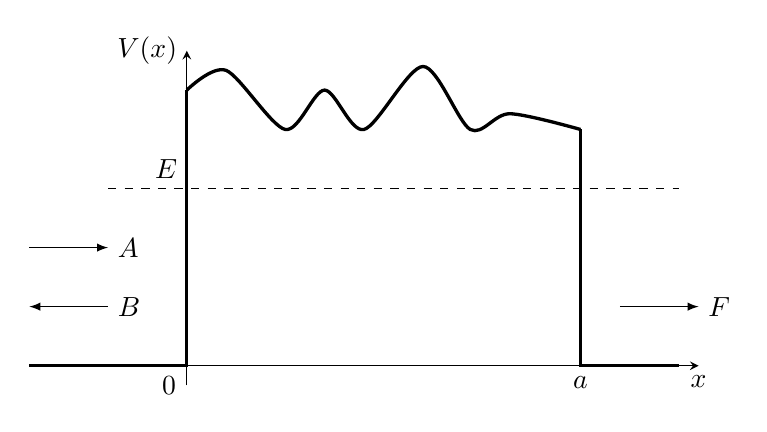
\begin{tikzpicture}
\draw[-stealth] (-0.5,0) -- (6.5,0)node[below]{$x$};
\draw[-stealth] (0,-0.25) -- (0,4)node[left]{$V(x)$};
%\draw[very thick](-2,0) -- (0,0) -- (0,3) to [out=30,in=180] ++(0.5,0) to [out=0,in=180] ++(0.75,-0.25) to [out=0,in=180] +%+(1,0.5) to [out=0,in=180] (5,3.5) -- (5,0)node[below]{$a$}-- (6,0);
\draw[very thick](-2,0) -- (0,0) node[below left]{$0$}-- (0,3.5) (5,3)--(5,0)node[below]{$a$}--(6.25,0);
\draw[very thick] plot [smooth] coordinates {(0,3.5)(0.5,3.75)(1.25,3)(1.75,3.5)(2.25,3)(3,3.8)(3.6,3)(4.1,3.2)(5,3)};
\draw[dashed](-1,2.25)--(6.25,2.25);
\draw[-latex](-2,1.5)--++(1,0)node[right]{$A$};
\draw[latex-](-2,0.75)--++(1,0)node[right]{$B$};
\draw[-latex](5.5,0.75)--++(1,0)node[right]{$F$};
\draw(0,2.25)node[above left]{$E$};
\end{tikzpicture}
\caption{موڑے دار بالائی سطح کے   مستطیلی رکاوٹ سے بکھراو۔}
\label{شکل_وکب_مستطیلی_رکاوٹ}
\end{figure}

ایک مثال کے طور پر ایک مستطیلی رکاوٹ جس کی بالائی سطح غیر ہموار ہ (شکل \حوالہ{شکل_وکب_مستطیلی_رکاوٹ}) سے بکھراو کا مسئلہ پر غور کریں۔ درکاوٹ کے بائیں جانب \عددی{x<0} 
\begin{align}
	\psi(x)=Ae^{ikx}+Be^{-ikx}.
\end{align}
جہاں \عددی{A} آمدی حیطہ اور \عددی{B} منعکس حیطہ ہے جبکہ \عددی{k\equiv\sqrt{2mE}/\hslash} ہے \حوالہء{حصہ \num{2.5}} دیکھیں۔ دکاوٹ کے دائیں جانب \عددی{x>a}
\begin{align}
	\psi(x)=Fe^{ikx};
\end{align}
\عددی{F} ترسیلی حیطہ جبکہ ترسیلی احتمال درج ذیل ہوگا
\begin{align}
	T=\frac{\abs{F}^{2}}{\abs{A}^{2}}.
\end{align}
سرنگزنی خطہ \عددی{0\leq x\leq a} میں ونزل، کرامرز، برلوان تخمین درج ذیل دیگی
\begin{align}
	\psi(x)\cong\frac{C}{\sqrt{\abs{p(x)}}}e^{\frac{1}{\hslash}\int^{x}_{0}\abs{p(x')}\dif x'}+\frac{D}{\sqrt{\abs{p(x)}}}e^{-\frac{1}{\hslash}\int^{x}_{0}\abs{p(x')}\dif x'}.
\end{align}

\begin{figure}
\centering
\begin{tikzpicture}
\draw[-stealth] (-2.75,0) -- (6,0)node[below]{$x$};
%\draw[-stealth] (0,-0.25) -- (0,4)node[left]{$V(x)$};
\draw[-stealth](-360/200,0) -- (-360/200,1) node[pos=0.5, fill=white]{$A$};
\draw[thick,domain=-560:0] ({\x/200},{cos(\x)});
\draw[thick,smooth](0,1) to [out = 0,in=160] ++ (1,-0.25) to [out=-20,in=170] ++ (2,-0.55);
\draw[thick,domain=0:900] plot[smooth] ({3+\x/400},{-0.1+0.3*cos(\x)});
\draw[dashed](0,0) -- (0,1.25) (1,1) -- (-2.25,1); 
\draw[](0,0.1)--++(0,-0.2) node[below]{$0$};
\draw[dashed](2.9,0) -- (2.9,0.5) (2.9,0.2) -- (5.25,0.2); 
\draw[](2.9,0.1)--++(0,-0.2) node[below]{$a$};
\draw[-stealth] (3.925,-0.5) -- (3.925,0);
\draw[stealth-] (3.925,0.2) -- (3.925,0.75) node[right]{$F$};
\end{tikzpicture}
\caption{اونچی اور چوڑی رکاوٹ سے بکھراو کے تفاعل  موج کی کیفی ساخت۔}
\label{شکل_وکب_اونچی_چوڑی}
\end{figure}


اگر رکاوٹ بہت بلند یا اور بہت چوڑا ہو یعنی جب سرنگزنی کا احتمال بہت کم ہو قوت نمائی بڑھتے جزو کا عددی سر \عددی{C} لاظماً چھوٹا ہوگا درحقیقت لامتناہی چوڑے رکاوٹ کی صورت میں یہ صفر ہوگا اور تفاعل موج کچھ  شکل \حوالہ{شکل_وکب_اونچی_چوڑی}  کے نقش پر ہوگی۔ غیر کلاسیکی خطہ پر قوتِ نمائی میں کل کمی 
\begin{align*}
	\frac{\abs{F}}{\abs{A}}\sim e^{-\frac{1}{\hslash}}\int^{a}_{0}\abs{p(x')}\dif x'.
\end{align*}
آمدی اور ترسیلی امواج کے اظافی حیطے تعین کرتا ہے لحاظہ درج ذیل ہوگا
\begin{align}
	\boxed{T\cong e^{-2\gamma},   \text{\RL{جہاں}}   \gamma\equiv\frac{1}{\hslash}\int^{a}_{0}\abs{p(x)}\dif x}.۔
\end{align}
\ابتدا{مثال}
\موٹا{ایلفا تحلیل کا نظریہ گامو۔} سن \num{1928} میں جارج گامو نے \حوالہء{مساوات \num{8.22}} استعمال کرتے ہوئے ایلفا تحلیل کی پہلی کامیاب وجہ پیش کی ایلفا تحلیل سے مراد چند مخصوص تابکار مرکزہ سے ایلفا ذرہ جو دو پروٹان اور دو نیوٹران پر مشتمل ہوتا ہے کا اخراج ہے۔ چونکہ ایلفا ذرہ مثبت بار \عددی{2e} کا حامل ہے لحاظہ جیسے ہی یہ مرکزہ سے اتنا دور ہوجاتا ہے کہ یہ مرکزی بندشی قوت سے فرار کر سکے مرکزہ کے باقی حصہ کا بار \عددی{Ze} اس کو برقی قوتِ دفع سے دور جانے پر مجبور کرے گا۔ تاہم اسکو پہلے اس مخفی رکاوٹ سے گزرنا ہوگا جو یورینیم کی صورت میں خارجی ایلفا ذرہ کی توانائی سے دوگنے سے بھی زیادہ ہے۔ گامو نے اس مخفی توانائی کو تخمینی طور  پر  شکل \حوالہ{شکل_وکب_گامو_نمونہ}  کے مخفیہ سے ظاہر کیا جس نے مرکزہ کے رداس \عددی{r_1} وصت تک مرکزی قوتِ کشش کو متناہی چوکور کنواں سے ظاہر کیا گیا جس کو کولومب قوتِ دفع کی دم کے ساتھ جوڑا گیا ہے۔ گامو نے کوانٹم سرنگزنی کو ایلفا ذرہ کی فرار کی وجہ کرار دیا یوں پہلی بار کوانٹم میکانیات کا اطلاق مرکزوی طبیعیات پر کیا گیا۔

\begin{figure}
\centering
\begin{tikzpicture}[declare function={f(\x)= 1/(\x);}]
\pgfmathsetmacro{\E}{f(4)}
\begin{axis}[axis lines=middle,xlabel={$r$},ylabel={$V(r)$}, xtick={1,4},
 xticklabels={\rlap{$\, r_1$} ,$r_2$, $0$}, ytick={-0.5,\E}, yticklabels={$-V_0$,$E$}, ylabel style={at={(current axis.above origin)},anchor=east},xlabel style={at={(current axis.right of origin)},anchor=north east},enlargelimits]
\addplot [thick,domain=1:5]{f(x)}node[pos=0.5,pin={45:{\RL{کولمب دفع}}}]{};
\addplot[thick,]coordinates{({1},{f(1)})(1,-0.5)(0,-0.5)};
\addplot[thick,]coordinates{(0,\E)(5,\E)};
\addplot[]coordinates{(0.75,-0.5)}node[pin={45:{\RL{مرکزوی بندش}}}]{};
\end{axis}
\end{tikzpicture}
\caption{تابکار مرکزی میں الفا ذرہ کی مخفی توانائی کا گامو نمونہ۔}
\label{شکل_وکب_گامو_نمونہ}
\end{figure}


اگر خارجی ایلفا ذرے کی توانائی \عددی{E} ہو تب بیرونی واپسی نقطہ \عددی{r_2} درج ذیل تعین کرے گا
\begin{align}
	\frac{1}{4\pi\epsilon_{0}}\frac{2Ze^{2}}{r_{2}}=E.
\end{align}
ظاہر ہے \حوالہء{مساوات \num{8.22}} میں قوت نما \عددی{\gamma} درج ذیل ہوگا
\begin{align*}
	\gamma=\frac{1}{\hslash}\int^{r_{2}}_{r_{1}}\sqrt{2m\Big(\frac{1}{4\pi\epsilon_{0}}\frac{2Ze^{2}}{r}-E\Big)}\dif r=\frac{\sqrt{2mE}}{\hslash}\int^{r_{2}}_{r_{1}}\sqrt{\frac{r_{2}}{r}-1}\dif r.
\end{align*}
اس تکمل میں \عددی{r\equiv r_2\sin^2u} پُر کرتے ہوئے نتیجہ حاصل کیا جاسکتا ہے
\begin{align}
	\gamma=\frac{\sqrt{2mE}}{\hslash}\left[r_{2}\left(\frac{\pi}{2}-\sin^{-1}\sqrt{\frac{r_{1}}{r_{2}}}\right)-\sqrt{r_{1}(r_{2}-r_{1})}\right].
\end{align}
عام طور پر \عددی{r_1\ll r_2} ہوگا لحاظہ ہم چھوٹے زاویوں کے تخمین \عددی{\sin\epsilon\cong\epsilon} استعمال کر کے نتیجہ کی سادہ روپ حاصل کرتے ہیں
\begin{align}
	\gamma\cong\frac{\sqrt{2mE}}{\hslash}\left[\frac{\pi}{2}r_{2}-2\sqrt{r_{1}r_{2}}\right]=K_{1}\frac{Z}{\sqrt{E}}-K_{2}\sqrt{Zr_{1}}.
\end{align}
جہہاں 
\begin{align}
	K_{1} \equiv \left(\frac{e^{2}}{4\pi\epsilon_{0}}\right)\frac{\pi\sqrt{2m}}{\hslash}= \SI{1.980}{\mega\electronvolt^{1/2}},
\end{align}
اور درج ذیل ہوگا
\begin{align}
	K_{2} \equiv \left(\frac{e^{2}}{4\pi\epsilon_{0}}\right)^{1/2}\frac{4\sqrt{m}}{\hslash}= \SI{1.485}{\femto\meter^{-1/2}}.
\end{align}
ایک عمومی مرکزہ کی جسامت تقریباً ایک \si{\femto\meter} \SI{e-15}{\meter} ہوتی ہے۔

اگر ہم مرکزہ کے اندر ایلفا ذرہ کو محسور تصور کریں اور کہیں کہ اسکی اوسط سمتی رفتار \عددی{v} ہے تب دیواروں کے ساتھ تصادم کے بیچ اوسط وقفہ تقریباً \عددی{2r_1/v} ہوگا لحاظہ تصادم کا تعدد \عددی{v/2r_1} ہوگا۔ ہر تصادم پر فراق ہونے کا احتمال \عددی{e^{-2\gamma}} ہے لحاظہ اکایئ وقت میں اخراج کا احتمال \عددی{(v/2r_1)e^{-2\gamma}} ہوگا اور یوں ولدہ مرکزہ کا عرصہ حیات تقریباً درج ذیل ہوگا
\begin{align}
	\tau=\frac{2r_{1}}{v} e^{2\gamma}.
\end{align}
بدقسمتی سے ہم \عددی{v} نہیں جانتے ہیں لیکن اس سے زیادہ فرق نہیں پڑتا ہے چونکہ ایک تابکار مرکزہ سے اور دوسرے تابکار مرکزہ کے بیچ قوتِ نمائی جزضربی پچیس رتبی مقدار تک تبدیل ہوتا ہے جس کے سامنے \عددی{v} کی تبدیلی قابلِ نظرانداز ہے۔ بالخصوص عرصہ حیات کی تجرباتی پیمائشی قیمتوں کو \عددی{1/\sqrt{E}} کے ساتھ ترسیم کرنے سے ایک خوبصورت سیدھا خط \حوالہء{شکل \num{8.6}} حاصل ہوتا ہے جو عین \حوالہء{مساوات \num{8.25} اور \num{8.28}} کے تحت ہوگا۔
\انتہا{مثال}
\ابتدا{سوال}
ایک متناہی چوکور رکاوٹ جس کی انچائی \عددی{V_0>E} اور چوڑائی \عددی{2a} ہو سے ایک ایسا ذرہ جس کی توانائی \عددی{E} ہو کی تخمینی ترسیمی احتمال \حوالہء{مساوات \num{8.22}} استعما کرتے ہوئے حاصل کریں۔ اپنے جواب کا موانہ بلکل ٹھیک نتیجہ \حوالہء{سوال \num{2.33}} کے ساتھ کریں۔
\انتہا{سوال}
\ابتدا{سوال}
\حوالہء{مساوات \num{8.25} اور \num{8.28}} استعمال کرتے ہوئے \عددی{U^{238}} اور \عددی{Po^{212}} کے عرصہ حیات تلاش کریں۔ تمام مرکزہ میں مرکزوی مادہ کی کثافت تقریباً مستقل ہوتی ہے لحاظہ \عددی{(r_1)^3} اور \عددی{A} پروٹان اور نیوٹرانوں کی تعدادوں کا مجموعہ تقریباً برابر ہوںگے۔ تجرباتی طور پر درج ذیل حاصل کیا گیا ہے
\begin{align}
	r_{1}\cong(\SI{1.07}{\femto\meter})A^{1/3}.
\end{align}
خارج شدہ ایلفا ذرہ کی توانائی کلیہ آئنسٹائن \عددی{E=mc^2} سے اغز کیا جاسکتا ہے
\begin{align}
	E=m_{p}c^{2}-m_{d}c^{2}-m_{\alpha}c^{2}.
\end{align}
جہاں \عددی{m_p} ولدہ مرکزہ کی کمیت \عددی{m_d} بیٹی مرکزہ کی کمیت اور \عددی{m_\alpha} ایلفا ذرہ یعنی \عددی{He^4} مرکزہ کی کمیت ہے۔ یہ دیکھنے کی خاطر کہ بیٹی مرکزہ کیا ہوگا یاد رکھیں کہ ایلفا ذرہ دو پروٹان اور دو نیوٹران لیکر فرار ہوتا ہے لحاظہ \عددی{Z} سے دو منفی کریں اور \عددی{A} سے چار منفی کریں گے۔ حاصل جوابات استعمال کرتے ہوئے دوری جدول سے کیمیائی انصر تعین کریں۔ سمتی رفتار \عددی{v} کی اندازاً قیمت \عددی{E=(1/2)m_\alpha v^2} سے حاصل کریں یہ مرکزہ کے اندر منفی مخفی توانائی کو نظرانداز کرتا ہے لحاظہ \عددی{v} کی قیمت اصل سے زیادہ دیگا تاہم اس مرحلہ پر ہم صرف اتنا ہی کر سکتے ہیں۔ اتفاقی طور پر ان کیمیائی اناصر کی تجربہ سے حاصل عرصہ حیات بالترتیب \عددی{6\times10^9} سال اور \SI{0.5}     {\micro\second} ہے۔
\انتہا{سوال}
%=======================



\حصہ{کلیات   پیوند}
اب تک کے بحس و فکر میں میں فرض کرتا رہا کہ مخفی کنواں یا رکاوٹ کی دیواریں انتصابی تھیں جس کی بنا پر بیرونی حل آسان اور سرحدی شرائط سادہ تھے۔ درحقیقت ہمارے بنیادی نتائج \حوالہء{مساوات \num{8.16} اور \num{8.22}} اس صورت بھی کافی حد تک دوست ہوںگے جب کناروں کی ڈھلان اتنی زیادہ نہ ہو یقیقناً نظریہ گامو میں ایسی ہی صورت پر انکا اطلاق کیا گیا۔ بہر حال ہم نقطہ واپسی \عددی{E=V} جہاں کلاسیکی اور غٖیر کلاسیکی خطے ایک دوسرے  کے ساتھ جڑتے ہیں اور ونزل، کرامرز، برلوان تخمین ناقابلِ استعمال ہوتی ہے پر تفاعل موج کا قریبی مطالعہ کرنا چاہیں گے۔ اس حصہ میں میں مکید حال مسئلہ  (شکل \حوالہ{شکل_وکب_کلاسیکی_مقید_خطہ})  کو دیکھتا ہوں،  آپ مسئلہ بکھراو ( \حوالہء{سوال \num{8.10}}) حل  کر سکتے ہیں۔
\begin{figure}
\centering
\begin{tikzpicture}
\fill[lgray] (-1,0.5) rectangle (1,3.75);
\draw[-stealth](-3,-0.5) -- (3.5,-0.5) node[below]{$x$};
\draw[-stealth](0,-0.75) -- (0,4) node[left]{$V(x)$};
\draw[] (-2.75,2.125) -- (2.75,2.125) node[right]{$E$};
\draw[name path=a,decoration={random steps,segment length=0.5mm,amplitude=0.5pt},decorate](-1,0.5) -- (-1,3.75);
\draw[name path=b,decoration={random steps,segment length=0.5mm,amplitude=0.5pt},decorate](1,0.5) -- (1,3.75);
\draw[decoration={brace,amplitude=5pt,raise=4pt, mirror,aspect=0.3},decorate] (-1,0.5) -- (1,0.5) node[midway,below left,yshift=-12pt]{\RL{پیوندکار خطہ}};
\draw[](0,2.125) node[pin={[pin distance=1.25cm]135:{\RL{نقطہ واپسیں}}}]{} --++ (45:2) node[pos=1,pin={10:{\RL{خط بند مخفیہ}}}]{};
\draw[](0,2.125) --++ (-135:2);
\draw[thick] (0,2.125) to [out=45,in=180] (2,3);
\draw[thick] (0,2.125) to [out=-135,in=0] (-2,1.25);
\draw[] (-2,-0.75) -- (-0.25,-0.75) node[pos=0.5,below]{\RL{کلاسیکی خطہ}}; 
\draw[] (+2,-0.75) -- (+0.25,-0.75) node[pos=0.5,below]{\RL{غیر کلاسیکی خطہ}}; 
\end{tikzpicture}
\caption{دائیں ہاتھ نقطہ واپسیں کو  وضاحت سے دکھایا گیا ہے۔}
\label{شکل_وکب_نقطہ_واپسیں_وضاحت}
\end{figure}


اپنی آسانی کی خاطر ہم محور کو یوں رکھتے ہیں کہ دائیں ہاتھ کا نقطہ واپسی \عددی{x=0} پر واقعہ ہو (شکل \حوالہ{شکل_وکب_نقطہ_واپسیں_وضاحت})۔ ونزل، کرامرز، برلوان تخمین میں درج ذیل ہوگا
\begin{align}
	\psi (x) \cong
	\begin{cases}
		\frac{1}{\sqrt{p(x)}}\left[B e^{\frac{i}{h} \int^{0}_{x} p(x^{'}) \dif x^{'}} + C e^{- \frac{i}{h} \int^{0}_{x} p(x^{'}) \dif x^{'}}\right] ,& x \textless 0 \text{\RL{اگر}}, \\
		\frac{1}{\sqrt{\abs{p(x)}}} D e^{- \frac{1}{h} \int^{x}_{0}} \abs{p(x^{'})} \dif x^{'},& x \textgreater 0 \text{\RL{اگر}}.
	\end{cases}
\end{align}
یہ فرض کرتے ہوئے تمام \عددی{x>0} \عددی{E} سے \عددی{V(x)} بڑا ہوگا ہم اس خطہ میں مثبت قوت نمائی کو خارج کرسکتے ہیں چونکہ \عددی{x\to\infty} کرنے سے یہ بے قابو بڑھتا ہے۔ ہمارا کام ان دو حالوں کو سرحد پر ایک دوسرے کے ساتھ جوڑنا ہے تاہم یہاں ہمیں شدید مشکلات کا سامنا پیش آتا ہے۔ ونزل، کرامرز، برلوان تخمین نے نقطہ واپسی جہاں \عددی{p(x)\to0} ہوگا \عددی{\psi} کی قیمت لامتناہی تک پہنچتی ہے۔ حقیقی تفاعل موج یقیناً ایسا رویہ نہیں رکھتا ہے اور جیسا کہ ہمارا گمان تھا ونزل، کرامرز، برلوان تخمین نقطہ واپسی کی پڑوس میں ناقابلِ استعمال ہوتا ہے لیکن اجازتی توانائیواں کو نکات واپسی پر سرحدی شرائط تعین کرتی ہیں۔ ہم ایک ایسا پیوندکار تفاعل موج لیتے ہیں جو نقطہ واپسی کو ڈھانپ کر دونوں اطراف کے ونزل، کرامرز، برلوان تخمین حل کو ایک دوسرے کے ساتھ پیوند کرتا ہو۔

چونکہ ہمیں پیوندکار تفاعل موج \عددی{\psi_p} صرف ممدہ کی پڑوس میں چاہیئے لحاظہ ہم اس مخفیہ کو سیدھی لکیر 
\begin{align}
	V(x) \cong E + V'(0)x,
\end{align}
سے تخمین کر کے اس خطی \عددی{V} کے لیئے شروڈنگر مساوات حل کرتے ہیں
\begin{align*}
	-\frac{\hslash^{2}}{2m} \frac{\dif^{2}\psi_{p}}{\dif x^{2}} +[E+V'(0)x]\psi_{p}=E\psi_{p},
\end{align*}
یا 
\begin{align}
	\frac{\dif^{2} \psi_{p}}{\dif x^{2}} = \alpha^{3} x\psi_{p},
\end{align}
جہاں درج ذیل ہے
\begin{align}
	\alpha\equiv\left[\frac{2m}{\hslash^{2}} V'(0)\right]^{1/3}.
\end{align}
درج ذیل متعارف کر کے ہم ان \عددی{\alpha} کو غیر تابع متغیر میں زن کرسکتے ہیں
\begin{align}
	z\equiv\alpha x,
\end{align}
لحاظہ درج ذیل ہوگا
\begin{align}
	\frac{\dif^{2}\psi_{p}}{\dif z^{2}}=z\psi_{p}.
\end{align}
یہ مساوات ایری ہے جس کے حل تفاعلات ایر کہلاتے ہیں چونکہ مساوات ایری دو رتبی تفرقی مساوات ہیں لحاظہ دو خطی غیر تابع ایری تفاعالات \عددی{Ai(z)} اور \عددی{Bi(z)} پائے جاتے ہیں۔
\begin{table}[h!]
\centering
\caption{ایری تفاعلات کے چند خواص}
\label{table:1}
\begin{tabular}{|c c|}
\hline
تفریقی مساوات: & $\frac{\dif^2y}{\dif z^2}=zy$\\
حل: & ایری تفاعالات کے خطی مجموعہ $Ai(z)$ اور $Bi(z)$ \\
تکملی روپ: & 
{$\begin{aligned}
Ai(z)&=\frac{1}{\pi}\int_{0}^{\infty}\cos\left(\frac{s^3}{3}+sz\right)\dif s \\
Bi(z)&=\frac{1}{\pi}\int_{0}^{\infty}\left[e^{-\frac{s^3}{3}+s}+\sin\left(\frac{s^3}{3}+sz\right)\right]\dif s
\end{aligned}$}\\
\hline
\end{tabular}
\end{table}
ان کا تعلق رتبہ \عددی{1/3} کے بیسل تفاعلات کے ساتھ ہے ان کے چند خواص \حوالہء{جدول \num{8.1}} میں دیئے گئے ہیں جبکہ \حوالہء{شکل \num{8.8}} میں انہیں ترسیم کیا گیا ہے ظاہر ہے کہ پیوندکار تفاعل موج \عددی{Ai(z)} اور \عددی{Bi(z)} کا خطی جوڑ 
\begin{align}
	\psi_{p}(x) = aAi(\alpha x)+ bBi(\alpha x).
\end{align}
ہوگا۔ جہاں \عددی{a} اور \عددی{b} مناسب مستقلات ہیں۔

\begin{figure}
\centering
\begin{tikzpicture}
\fill[lgray] (-2.5,0.5) rectangle (-1.5,3.75);
\fill[lgray] (1.5,0.5) rectangle (2.5,3.75);
\draw[-stealth](-3,0.5) -- (3.5,0.5) node[below]{$x$};
\draw[](0,-0.65) -- (0,4);
\draw[name path=a,decoration={random steps,segment length=0.5mm,amplitude=0.5pt},decorate](-2.5,0.5) -- (-2.5,3.75);
\draw[name path=b,decoration={random steps,segment length=0.5mm,amplitude=0.5pt},decorate](-1.5,0.5) -- (-1.5,3.75);
\draw[name path=a,decoration={random steps,segment length=0.5mm,amplitude=0.5pt},decorate](2.5,0.5) -- (2.5,3.75);
\draw[name path=b,decoration={random steps,segment length=0.5mm,amplitude=0.5pt},decorate](1.5,0.5) -- (1.5,3.75);
\draw[decoration={brace,amplitude=5pt,raise=4pt, mirror},decorate] (-2.5,0.5) -- (-1.5,0.5) node[midway,below,yshift=-12pt]{\RL{جزوی منطبق خطہ}};
\draw[decoration={brace,amplitude=5pt,raise=4pt, mirror},decorate] (1.5,0.5) -- (2.5,0.5) node[midway,below,yshift=-12pt]{\RL{جزوی منطبق خطہ}};
\draw[] (-2.5,-0.75) -- (2.5,-0.75) node[pos=0.5,below]{\RL{پیوندکار خطہ}};
\draw[](0,0.5) node[fill=black,circle,inner sep=1.5pt]{} node[pin={[text centered, text width=1cm]45:{\RL{نقطہ واپسیں}}}]{};
\draw[stealth-stealth] (-2.5,2.5) -- (2.5,2.5) node[pos=0.6,fill=white]{$\psi_p$};
\draw[stealth-] (-1.5,3) -- (-3.75,3) node[above right]{$\psi_{WKB}$};
\draw[stealth-] (1.5,3) -- (3.75,3) node[above left]{$\psi_{WKB}$};
\end{tikzpicture}
\caption{پیوندکار خطہ اور دو  منطبق  خطے۔}
\label{شکل_وکب_پیوندکار_منطبق}
\end{figure}

اب \عددی{\psi_p} مبدہ کی پڑوس میں تخمینی تفاعل موج ہے ہم نے مبدہ کے دونونں اطراف قریبی مشترکہ خطہ میں \عددی{\psi_p} کو ونزل، کرامرز، برلوان تخمین حلوں کے ساتھ ہم پلو بنانا ہوگا ( شکل \حوالہ{شکل_وکب_پیوندکار_منطبق}  دیکھیں)۔ دونوں اطراف کے مشترک خطے نقطہ واپسی کے اتنی قریب ہیں کہ خطی مخفیہ \عددی{\psi_p} کافی حد تک درست ہوگا لحاظہ \عددی{\psi_p} اصل تفاعل موج کا بہترین تخمین ہوگا لیکن ساتھ ہی یہ مشترکہ خطے نقطہ واپسی سے اتنی فاصلہ پر ہیں کہ ونزل، کرامرز، برلوان تخمین پر بھروسہ کیا جا ساکتا ہے۔ مشترکہ خطوں میں \حوالہء{مساوات \num{8.32}} کارآمد ہوگا لحاظہ \حوالہء{مساوات \num{8.34}} کی لامتیت میں درج ذیل ہوگا
\begin{align}
	p(x) \cong \sqrt{2m(E-E-V'(0)x)} =\hslash\alpha^{3/2}\sqrt{-x}.
\end{align}
بالخصوص مشترکہ خطہ دو میں درج ذیل ہوگا 
\begin{align*}
	\int^{x}_{0} \abs{p(x')} \dif x' \cong \hslash\alpha^{3/2} \int^{x}_{0}\sqrt{x'}\dif x'=\frac{2}{3}\hslash(\alpha x)^{3/2},
\end{align*}
لحاظہ ونزل، کرامرز، برلوان تخمین تفاعل موج \حوالہء{مساوات \num{8.31}} درج ذیل لکھی جاسکتی ہے
\begin{align}
	\psi(x)\cong\frac{D}{\sqrt{\hslash}\alpha^{3/4}x^{1/4}} e^{-\frac{2}{3}(\alpha x)^{3/2}}.
\end{align}
بڑی \عددی{z} کی صورت میں ایری تفاعلات کی متقاربی روپ \حوالہء{جدول \num{8.3}} لیتے ہوئے مشترکہ خطہ دو میں پیوند کار تفعال موج \حوالہء{مساوات \num{8.37}} درج ذیل روپ اختیار کرتی ہے
\begin{align}
	\psi_{p}(x)\cong \frac{a}{2\sqrt{\pi}(\alpha x)^{1/4}} e^{-\frac{2}{3}(\alpha x)^{3/2}} +\frac{b}{\sqrt{\pi}(\alpha x)^{1/4}} e^{\frac{2}{3}(\alpha x)^{3/2}}.
\end{align}
دونوں حلوں کے موازنہ سے درج ذیل لکھا جاسکتا ہے
\begin{align}
	a=\sqrt{\frac{4\pi}{\alpha\hslash}}D,&& \text{\RL{اور}}&& b=0.
\end{align}
ہم یہی کچھ مشترکہ خطہ ایک کے لیئے بھی کرتے ہیں اب بھی \حوالہء{مساوات \num{8.38}} ہمیں \عددی{p(x)} دیگا تاہم اس بار \عددی{x} منفی ہوگا جس کے تحت درج ذیل ہوگا
\begin{align}
	\int^{0}_{x} p(x')\dif x' \cong \frac{2}{3}\hslash(-\alpha x)^{3/2}
\end{align}
اور ونزل، کرامرز، برلوان تخمین تفاعل موج \حوالہء{مساوات \num{8.31}} درج ذیل ہوگا
\begin{align}
	\psi(x)\cong\frac{1}{\sqrt{\hslash}\alpha^{3/4}(-x)^{1/4}} \left[B e^{i\frac{2}{3}(-\alpha x)^{3/2}} + C e^{-i\frac{2}{3}(-\alpha x)^{3/2}}\right].
\end{align}
ساتھ ہی بہت بڑی منفی \عددی{z} کے لیئے ایری تفاعل کی متقارب روپ \حوالہء{جدول \num{8.1}} استعمال کرتے ہوئے پیوندی تفاعل \حوالہء{مساوات \num{8.37}} جس میں \عددی{b=0} لیا گیا ہو درج ذیل ہوگی
\begin{align}
	\psi_{p}(x) &\cong\frac{a}{\sqrt{\pi}(-\alpha x)^{1/4}} \sin \left[\frac{2}{3}(-\alpha x)^{3/2}+\frac{\pi}{4}\right]\nonumber \\
	&=\frac{a}{\sqrt{\pi}(-\alpha x)^{1/4}}\frac{1}{2i}\left[e^{i\pi/4} e^{i\frac{2}{3}(-\alpha x)^{3/2} - e^{-i\pi/4} e^{-i\frac{2}{3}(-\alpha x)^{3/2}}} \right].
\end{align}
مشترکہ خطہ ایک میں ونزل، کرامرز، برلوان تخمین اور پیوندی تفاعلات موج کے موازنے سے درج ذیل حاصل ہوگا 
\begin{align*}
	\frac{a}{2i\sqrt{\pi}} e^{i\pi/4}=\frac{B}{\sqrt{\hslash\alpha}}&& \text{\RL{اور}}&& \frac{-a}{2i\sqrt{\pi}}e^{-i\pi/4}=\frac{C}{\sqrt{\hslash\alpha}}.
\end{align*}
جس میں \عددی{a} کی قیمت \حوالہء{مساوات \num{8.41}} سے پر کر کے درج ذیل حاصل ہوگا
\begin{align}
	B=-ie^{i\pi/4}D,&&\text{\RL{اور}}&&C=ie^{-i\pi/4}D.
\end{align}
انہیں کلیات جوڑ کہتے ہیں جو نقطہ واپسی کے دونوں اطراف ونزل، کرامرز، برلوان تخمین حلوں کو ایک دوسرے کے ساتھ پیوند کرتے ہیں۔ پیوندی تفاعل موج کا کام نقطہ واپسی پر پیدا درز کو ڈھانپنا تھا۔ اس کے آگے ضرورت پیش نہیں آئے گی سب چیزوں کو واحد ایک معمولزنی مستقل \عددی{D} کی صورت میں بیان کر کے نقطہ واپسی کو واپس مبدہ سے اختیاری نقطہ \عددی{x_2} منتقل کرتے ہوئے ونزل، کرامرز، برلوان تفاعل موج \حوالہء{مساوات \num{8.31}} درج ذیل روپ اختیار کرتی ہے
\begin{align}
	\psi(x)\cong
	\begin{cases}
		\frac{2D}{\sqrt{p(x)}} \sin\left[\frac{1}{\hslash}\int^{x_{2}}_{x} p(x') \dif x' +\frac{\pi}{4} \right], & x\textless x_{2} \text{\RL{اگر}}; \\
		\frac{D}{\sqrt{\abs{p(x)}}} \exp\left[\frac{1}{\hslash}\int^{x}_{x_{2}} \abs{p(x')}\dif x' \right], & x\textgreater x_{2} \text{\RL{اگر}}.
	\end{cases}
\end{align}
\ابتدا{مثال}
\موٹا{ایک انتصابی دیوار والا مخفیہ کنواں۔} فرض کریں ایک مخفیہ کنویں کی \عددی{x=0} پر انتصابی دیوار جبکہ دوسری دیوار ڈھلان  ہو (شکل \حوالہ{شکل_وکب_ایک_دیوار_کنواں})۔ ایسی صورت میں \عددی{\psi(0)=0} ہوگا لحاظہ \حوالہء{مساوات \num{8.46}} کے تحت 
\begin{align*}
	\frac{1}{\hslash}\int^{x_{2}}_{0} p(x)\dif x+\frac{\pi}{4}=n\pi,&&n=(1,2,3,\dots).
\end{align*}
یا درج ذیل ہوگا۔
\begin{align}
	\int^{x_{2}}_{0}p(x)\dif x=\left(n-\frac{1}{4}\right)\pi\hslash
\end{align}

\begin{figure}
\centering
\begin{tikzpicture}
\fill[path fading=west,color=lgray] (-0.25,0) rectangle (0,3.75);
\draw[-stealth] (-0.5,0) -- (5.75,0)node[below]{$x$};
\draw[-stealth] (0,-0.25) -- (0,4)node[left]{$V(x)$};
\draw[very thick, name path=a] (0,3.5) -- (0,0.25) to [out=0,in=180] ++ (2,1) to [out=0,in=-120] ++ (2,1) to [out=60,in=-160] ++ (1,1); 
\draw[name path=b](0,2) node[left,xshift={-0.5em}]{$E$} -- (5,2);
\draw[dashed,name intersections={of={a and b}}] (intersection-2) -- ($(0,0)!(intersection-2)!(5,0)$) node[below]{$x_2$};
\end{tikzpicture}
\caption{ایک  انتصابی  دیوار والا مخفیہ کنواں۔}
\label{شکل_وکب_ایک_دیوار_کنواں}
\end{figure}

مثلاً نصف ہارمونی مرتعش 
\begin{align}
	V(x)=
	\begin{cases}
		\frac{1}{2}m\omega^{2}x^{2}, & x\textgreater 0 \text{\RL{اگر}}, \\
		0, &\text{\RL{دیگر صورت}}
	\end{cases}
\end{align}
پر غور کریں۔ اس صورت میں
\begin{align*}
	p(x)=\sqrt{2m[E-(1/2)m\omega^{2}x^{2}]}=m\omega\sqrt{x^{2}_{2}-x^{2}}.
\end{align*}
ہوگا۔ جہاں درج ذیل نوطہ واپسی ہے
\begin{align*}
	x_{2}=\frac{1}{\omega}\sqrt{\frac{2E}{m}}
\end{align*}
لحاظہ
\begin{align*}
	\int^{x_{2}}_{0} p(x)\dif x=m\omega\int^{x_{2}}_{0}\sqrt{x^{2}_{2}-x^{2}}\dif x=\frac{\pi}{4}m\omega x^{2}_{2}=\frac{\pi E}{2\omega}.
\end{align*}
اور کوانٹازنی شرط \حوالہء{مساوات \num{8.47}} درج ذیل دیگا
\begin{align}
	E_{n}=\left(2n-\frac{1}{2}\right)\hslash\omega=\left(\frac{3}{2}, \frac{7}{2}, \frac{11}{2},\dots\right)\hslash\omega.
\end{align}
اس مخصوص صورت میں ونزل، کرامرز، برلوان تخمین درحقیقت ٹھیک ٹھیک اجازتی توانائیاں دیتا ہے جو مکمل ہارمونی مرتعش کی طاق توانائیاں ہیں \حوالہء{سوال \num{2.42}} دیکھیں۔
\انتہا{مثال}


\ابتدا{مثال}
\موٹا{بغیر انتصابی دیواروں کا مخفیہ کنواں۔} اس نقطہ واپسی پر جہاں مخفیہ کی ڈھلوان اوپر رخ  (شکل \حوالہ{شکل_وکب_بالائی_جانب_نقطہ_واپسیں}-ا) ہوتی ہے \حوالہء{مساوات \num{8.46}} ونزل، کرامرز، برلوان تفاعلات موج کو پیوند کرتی ہے نیچے رخ ڈھلوانی نقطہ واپسی (شکل \حوالہ{شکل_وکب_بالائی_جانب_نقطہ_واپسیں}-ب)  پر انہی وجوہات کو بروہ ِکار لاتے ہوئے درج ذیل ہوگا \حوالہء{سوال \num{8.9}}
\begin{align}
	\psi(x)\cong
	\begin{cases}
		\frac{D'}{\sqrt{p(x)}} \exp\left[-\frac{1}{\hslash}\int^{x_{1}}_{x} \abs{p(x')}\dif x'\right],&x\textless x_{1} \text{\RL{اگر}}; \\
		\frac{2D'}{\sqrt{p(x)}} \sin\left[\frac{1}{\hslash}\int^{x}_{x_{1}}p(x')\dif x'+\frac{\pi}{4}\right],&x\textgreater x_{1} \text{\RL{اگر}}.
	\end{cases}
\end{align}
%
\begin{figure}
\centering
\begin{subfigure}{0.22\textwidth}
\centering 
\pgfmathsetmacro{\a}{70}
\pgfmathsetmacro{\b}{180-\a}
\begin{tikzpicture}
%\draw[-stealth] (0,0) -- (0.5,0)node[below]{$x$};
%\draw[-stealth] (0,0) -- (0,3)node[left]{$V(x)$};
\draw[] (-1,0) node[left]{$E$} -- (1,0);
\draw[dashed] (0,-1) node[below]{$x_2$} -- (0,1);
\draw[very thick, name path=a] (0,0) to [out=\a,in=-170] ++ (1,1); 
\draw[very thick, name path=a] (0,0) to [out=-\b,in=10] ++ (-1,-1); 
\end{tikzpicture}
\caption{}
\end{subfigure}\hfill
\begin{subfigure}{0.22\textwidth}
\centering 
\pgfmathsetmacro{\a}{70}
\pgfmathsetmacro{\b}{180-\a}
\begin{tikzpicture}
%\draw[-stealth] (0,0) -- (0.5,0)node[below]{$x$};
%\draw[-stealth] (0,0) -- (0,3)node[left]{$V(x)$};
\draw[] (-1,0) node[left]{$E$} -- (1,0);
\draw[dashed] (0,-1) node[below]{$x_1$} -- (0,1);
\draw[very thick, name path=a] (0,0) to [out=-\a,in=170] ++ (1,-1); 
\draw[very thick, name path=a] (0,0) to [out=\b,in=-10] ++ (-1,1); 
\end{tikzpicture}
\caption{}
\end{subfigure}\hfill
\begin{subfigure}{0.45\textwidth}
\centering 
\pgfmathsetmacro{\a}{70}
\pgfmathsetmacro{\b}{180-\a}
\begin{tikzpicture}
\draw[-stealth] (-1.5,-1.5) -- ++(0.5,0)node[below]{$x$};
\draw[-stealth] (-1.5,-1.5) -- ++(0,3)node[below left]{$V(x)$};
\draw[] (-1,0) node[left]{$E$} -- (3,0);
\draw[dashed] (0,-1) node[below]{$x_1$} -- (0,1);
\draw[dashed] (2,-1) node[below]{$x_2$} -- (2,1);
\draw[very thick, name path=a] (0,0) to [out=-\a,in=180] ++ (1,-1); 
\draw[very thick, name path=a] (0,0) to [out=\b,in=-10] ++ (-1,1); 
\draw[very thick, name path=a] (2,0) to [out=-\b,in=0] ++ (-1,-1); 
\draw[very thick, name path=a] (2,0) to [out=\a,in=-170] ++ (1,1); 
\end{tikzpicture}
\caption{}
\end{subfigure}
\caption{بالائی جانب ڈھلوان اور نیچے جانب ڈھلون نقطہ وپسیں۔}
\label{شکل_وکب_بالائی_جانب_نقطہ_واپسیں}
\end{figure}



بالخصوص مخفیہ کنویں (شکل \حوالہ{شکل_وکب_بالائی_جانب_نقطہ_واپسیں}-ج)  کی بات کرتے ہوئے اندرونی خطہ \عددی{(x_1<x<x_2)} میں تفاعل موج کو  
\begin{align*}
	\psi(x)\cong\frac{2D}{\sqrt{p(x)}} \sin\theta_{2}(x),&&\theta_{2}(x)\equiv \frac{1}{\hslash}\int^{x_{2}}_{x} p(x')\dif x'+\frac{\pi}{4},\text{\RL{جہاں}}
\end{align*}
لکھا جاسکتا ہے \حوالہء{مساوات \num{8.46}} یا درج ذیل لکھا جاسکتا ہے
\begin{align*}
	\psi(x)\cong\frac{-2D'}{\sqrt{p(x)}} \sin\theta_{1}(x),&&\theta_{1}(x)\equiv -\frac{1}{\hslash}\int^{x}_{x_{1}} p(x')\dif x'-\frac{\pi}{4}.
\end{align*}
\حوالہء{مساوات \num{8.50}}۔ ظاہر ہے کہ \عددی{\theta_2=\theta_1+n\pi} ہوگا جس سے درج ذیل حاصل ہوتا ہے
\begin{align}
	\boxed{\int^{x_{2}}_{x_{1}}p(x)\dif x=\left(n-\frac{1}{2}\right)\pi\hslash,\quad n=1,2,3,\dots\text{\RL{جہاں}}}
\end{align}
یہ کوانٹازنی شرط عمومی صورت کے دو ڈھلوان اطراف کے مخفیہ کنویں کی اجازتی توانائیاں تعین کرتا ہے دیہان رہے دو انتصابی دیواروں کے لیئے کلیہ \حوالہء{مساوات \num{8.16}} ایک انتصابی دیوار کے لیئے کلیہ \حوالہء{مساوات \num{8.47}} اور موجودہ کلیہ \حوالہء{مساوات \num{8.51}} میں صرف اُس عدد (\عددی{0, 1/4} یا \عددی{1/2}) کا فرق ہے جو \عددی{n}  سے منفی ہوتا ہے۔ چونکہ ونزل، کرامرز، برلوان تخمین بڑی \عددی{n} کی نیم کلاسیکی صورت میں بہترین کام کرتا ہے لحاظہ یہ فرق صرف دیکھاوے کی حد تک ہے بہر حال یہ نتیجہ انتہائی طاقتور ہے جس کو استعمال کرتے ہوئے شروڈنگر مساوات کیئے بغیر ایک سادہ تکمل کی قیمت حاصل کر کے ہم تخمینی اجازتی توانائیاں معلوم کر سکتے ہیں۔ تفاعل موج خود کہیں نہیں نظر آتا ہے۔
\انتہا{مثال}
\ابتدا{سوال}
زمین پر مکمل لچک کے ساتھ اُچھلتا ہوا کمیت \عددی{m} کی گیند کے کلاسیکی مسئلے کا مماثل کوانٹم میکانی مسئلے پر غور کریں۔

(الف) مخفی توانائی کیا ہوگی اس کو زمین سے بلندی \عددی{x} تفاعل لکھیں؟منفی \عددی{x} کی صورت میں مخفیہ لامتناہی ہوگا چونکہ گیند وہاں کبھی کبھی نہیں جاسکتا۔

(ب) اس مخفیہ کے لیئے مساوات شروڈنگر حل کر کے اپنے جواب کو مناسب ایری تفاعل کی روپ میں لکھیں چونکہ بڑی \عددی{z} کے لیئے \عددی{Bi(z)} بےقابو بڑھتا ہے لحاظہ اس کو رد کرنا ہوگا۔ تفاعل \عددی{\psi(x)} کو معمول پر لانے کی ضرورت نہیں۔

(ج) پہلی چار اجازتی توانائیوں کو تین معنی خیز ہندسوں تک \عددی{g=\SI{9.80}{\meter/\second\squared}} اور \عددی{m=\SI{0.100}{\kilogram}} لیکر حاصل کریں۔

(د) اس سکلی میدان میں ایک الیکٹران کی زمینی حال توانائی \عددی{\si{\electronvolt}} میں کتنی ہوگی؟ اوسطاً یہ الیکٹران زمین سے کتنی بلندی پر ہوگا؟ اشارہ: مسئلہ ویریل سے \عددی{\langle x\rangle} تعین کریں۔
\انتہا{سوال}
\ابتدا{سوال}
ونزل، کرامرز، برلوان تخمین استعمال کرتے ہوئے \حوالہء{سوال \num{8.5}} کی تھپکیاں کھاتے ہوئے گیند کا تجزیہ کریں۔

(الف) اجازتی توانائیاں \عددی{E_n} کو \عددی{m, g} اور \عددی{\hslash} کی صورت میں لکھیں۔

(ب) اب \حوالہء{سوال \num{8.5} (ج)} میں دی گئی مخصوص قیمتوں کو پُر کر کے ونزل، کرامرز، برلوان تخمین کی ابتدائی چار توانائیوں کا بلکل ٹھیک ٹھیک نتائج کے ساتھ موازنہ کریں۔

(ج) کوانٹم عدد \عددی{n} کتنا بڑا ہونا ہوگا کہ گیند اوسطاً زمین سے ایک میٹر کی بلندی پر ہو۔
\انتہا{سوال}
\ابتدا{سوال}
ہارمونی مرتعش کی اجازتی توانائیوں کو ونزل، کرامرز، برلوان تخمین سے حاصل کریں۔
\انتہا{سوال}
\ابتدا{سوال}
ہارمونی مرتعش جسکی زاویائی تعدد \عددی{\omega} ہو کی \عددی{n}ویں ساکن حال میں کمیت \عددی{m} کے ایک ذرہ پر غور کریں۔

(الف) نقطہ واپسی \عددی{x_2} تلاش کریں۔

(ب) نقطہ واپسی سے آپ کو کتنی بلندی \عددی{(d)} تک پہنچنا ہوگا کہ خطی مخفیہ \حوالہء{مساوات \num{8.32}} میں لیکن جس میں نقطہ واپسی \عددی{x_2} ہو خلل \عددی{1\percent} تک پہنچے گا یعنی اگر درج ذیل ہو
\begin{align*}
	\frac{V(x_{2}+d)-V_{lin}(x_{2}+d)}{V(x_{2})}=\num{0.01},
\end{align*}
تب \عددی{d} کیا ہوگا؟

(ج) جب تک \عددی{z\geq5} ہو \عددی{Ai(z)} کا متقارب روپ \عددی{1\percent} تک درست ہوگا۔ جزو (ب) میں حاصل کردہ \عددی{d} کے لیئے \عددی{n} کی ایسی کم سے کم قیمت تلاش کریں تاکہ \عددی{\alpha d\geq5} ہو۔ اس قیمت سے بڑی قیمت کے کسی بھی  \عددی{n} کے لیئے ایسا مسترکہ خطہ موجود ہوگا جس میں خطی مخفیہ \عددی{1\percent} تک کارآمد ہوگا اور بڑی \عددی{z} روپ کا ایری تفاعل بھی \عددی{1\percent} تک درست ہوگا۔
\انتہا{سوال}
\ابتدا{سوال}
نیچے رخ ڈھلوان کے نقطہ واپسی کے لیئے پیوندی کلیہ اخز کر کے \حوالہء{مساوات \num{8.50}} صفر کی تصدیق کریں۔
\انتہا{سوال}
\ابتدا{سوال}
مناسب پیوندی کلیات استعمال کر کے ڈھلوان  دیواروں کی رکاوٹ (شکل \حوالہ{شکل_وکب_ڈھلوانی_دیواروں_رکاوٹ}) سے بکھراو کے مسئلہ پر غور کریں۔ اشارہ: درج ذیل روپ کی ونزل، کرامرز، برلوان تفاعل موج لکھ کر آغاز کریں ۔
\begin{align}
	\psi(x)\cong
	\begin{cases}
		\frac{1}{\sqrt{p(x)}}\left[A e^{\frac{i}{\hslash}\int^{x_{1}}_{x}p(x')\dif x'}+B e^{-\frac{i}{\hslash}\int^{x_{1}}_{x}p(x')\dif x'}\right],& (x \textless x_{1}); \\
		\frac{1}{\sqrt{\abs{p(x)}}}\left[C e^{\frac{1}{\hslash}\int^{x}_{x_{1}}\abs{p(x')}\dif x'}+D e^{-\frac{1}{\hslash}\int^{x}_{x_{1}}\abs{p(x')}\dif x'}\right],& (x_{1} \textless x \textless x_{2}); \\
		\frac{1}{\sqrt{p(x)}}\left[F e^{\frac{i}{\hslash}\int^{x}_{x_{2}}p(x')\dif x'}\right],& (x \textgreater x_{2}).
	\end{cases}
\end{align}

\begin{figure}
\centering 
\begin{tikzpicture}
\pgfmathsetmacro{\a}{135}
\pgfmathsetmacro{\b}{180 - \a}
\draw[-stealth] (-3,0) -- (3,0)node[below]{$x$};
\draw[-stealth] (0,-0.25) -- (0,3)node[left]{$V(x)$};
\draw[name path=a] (-3,1.5) node[left]{$E$} -- (3,1.5);
\draw[very thick, name path=b] (-3,0.2) to [out=10,in=-\a] ++ (2,2) to [out=\b, in=0] (0,2.5) to [out=0,in=-180] ++ (0.5,0.25) to [out=0,in=170] (3,0.2);
\draw[dashed,name intersections={of={a and b}}] (intersection-1) -- ($(-3,0)!(intersection-1)!(3,0)$) node[below]{$x_1$}  (intersection-1) --++ (0,0.25);
\draw[dashed,name intersections={of={a and b}}] (intersection-2) -- ($(-3,0)!(intersection-2)!(3,0)$) node[below]{$x_2$}  (intersection-2) --++ (0,0.25);
\end{tikzpicture}
\caption{ڈھلوانی دیواروں والا رکاوٹ۔}
\label{شکل_وکب_ڈھلوانی_دیواروں_رکاوٹ}
\end{figure}

مستقل \عددی{C} کو صفر تصور نہ کریں۔ سرنگزنی احتمال \عددی{T=\abs{F}^2/\abs{A}^2} کا حساب کر کے دیکھائیں کہ بلند اور چوڑی رکاوٹ کی صورت میں اس سے \حوالہء{مساوات \num{8.22}} حاصل ہوگا۔
\انتہا{سوال}
\ابتدا{سوال}
عمومی قوت نمائی مخفیہ 
\begin{align*}
	V(x)=\alpha\abs{x}^{v},
\end{align*}
جہاں \عددی{v} ایک مثبت عدد ہے کی اجازتی توانائیوں کو ونزل، کرامرز، برلوان تخمین سے تلاش کریں۔ اپنے نتیجہ کو \عددی{v=2} جانچیں۔ جواب:
\begin{align}
	E_{n}=\alpha\left[(n-1/2)\hslash\sqrt{\frac{\pi}{2m\alpha}}\frac{\Gamma\left(\frac{1}{v}+\frac{3}{2}\right)}{\Gamma\left(\frac{1}{v}+1\right)}\right]^{\left(\frac{2v}{v+2}\right)}
\end{align}
\انتہا{سوال}
\ابتدا{سوال}
ونزل، کرامرز، برلوان تخمین استعمال کر کے \حوالہء{سوال \num{2.51}} کی مخفیہ کے لیئے مقید حال توانائی تلاش کریں۔ نتیجے کا ٹھیک ٹھیک جواب کے ساتھ موازنہ کریں۔ جواب: \عددی{-[(9/8)-(1/\sqrt{2})]\hslash^2a^2/m}
\انتہا{سوال}
\ابتدا{سوال}
کروی تشاکلی مخفیہ کے لیئے ہم رداسی حصہ \حوالہء{مساوات \num{4.37}} پر ونزل، کرامرز، برلوان تخمین کا اطلاق کر سکتے ہیں۔ \حوالہء{مساوات \num{8.47}} کی درج ذیل روپ کو \عددی{l=0} کی صورت میں استعمال کرنا معقول ہوگا 
\begin{align}
	\int^{r_{0}}_{0}p(r)\dif r=(n-1/4)\pi\hslash,
\end{align}
جہاں \عددی{r_0} نقطہ واپسی ہے یعنی ہم \عددی{r=0} کو لامتناہی دیوار تصور کرتے ہیں۔ اس کلیہ کو زیرِ استعمال لاتے ہوئے لوگردمی مخفیہ 
\begin{align*}
	V(r)=V_{0}\ln(r/a)
\end{align*}
کی اجازتی توانائیوں کی اندازاً قیمت تلاش کریں جہاں \عددی{V_0} اور \عددی{a} مستقلات ہیں۔ صرف \عددی{l=0} کی صورت پر غور کریں دیکھائیں کہ سطحوں کے بیچ فاصلوں کا انحصار کمیت پر نہیں ہوگا۔ جزوی جواب:
\begin{align*}
	E_{n+1}-E_{n}=V_{0}\ln\left(\frac{n+3/4}{n-1/4}\right).
\end{align*}
\انتہا{سوال}
\ابتدا{سوال}
ونزل، کرامرز، برلوان تخمین کی درج ذیل روپ
\begin{align}
	\int^{r_{2}}_{r_{1}}p(r)\dif r=(n-1/2)\pi\hslash
\end{align}
استعمال کر کے ہائڈروجن کی مکید حال توانائیوں کی اندازاً قیمت تلاش کریں۔ معصر مخفیہ \حوالہء{مساوات \num{4.38}} میں مرکز گریز جزو شامل کرنا مت بھولیں۔ درج ذیل تکمل مددگار ثابت ہو سکتا ہے
\begin{align}
	\int^{b}_{a}\frac{1}{x}\sqrt{(x-a)(b-x)}\dif x=\frac{\pi}{2}(\sqrt{b}-\sqrt{a})^{2}.
\end{align}
آپ دیکھیں گے کہ \عددی{n\gg l} اور \عددی{n\gg1/2} کی صورت میں آپ کو بوہر سطحیں ملیں گی۔ جواب:
\begin{align}
	E_{nl}\cong\frac{\SI{-13.6}{\electronvolt}}{[n-(1/2)+\sqrt{l(l+1)}]^{2}}.
\end{align}
\انتہا{سوال}
\ابتدا{سوال}
تشاکلی دوہرا  کنویں  (شکل \حوالہ{شکل_وکب_تشاکلی_دہرا_کنواں})  پر غور کریں۔ ہم \عددی{E<V(0)} والی مکید حالات میں دلچسپی رکھتے ہیں۔
\begin{figure}
\centering 
\begin{tikzpicture}
\pgfmathsetmacro{\a}{135}
\pgfmathsetmacro{\b}{180 - \a}
\draw[-stealth] (-3,0) -- (3.5,0)node[below]{$x$};
\draw[-stealth] (0,-0.25) -- (0,3)node[left]{$V(x)$};
\draw[name path=a] (-3,1) node[left]{$E$} -- (3,1);
\draw[very thick, name path=b] (0,1.5) to [out=0,in=180] (1,0) to [out=0, in=-100] (3,2.5)  (0,1.5) to [out=180,in=0] (-1,0) to [out=180, in=-90] (-3,2.5);
\draw[dashed,name intersections={of={a and b}}] (intersection-1) -- ($(-3,0)!(intersection-1)!(3,0)$) node[below]{$x_1$}  (intersection-1) --++ (0,0.25);
\draw[dashed,name intersections={of={a and b}}] (intersection-2) -- ($(-3,0)!(intersection-2)!(3,0)$) node[below]{$x_2$}  (intersection-2) --++ (0,0.25);
\end{tikzpicture}
\caption{تشاکلی دہرا کنواں؛ سوال \حوالہء{8.15}۔}
\label{شکل_وکب_تشاکلی_دہرا_کنواں}
\end{figure}


(الف) خطہ (i) \عددی{x>x_2}، (ii) \عددی{x_1<x<x_2} اور (iii) \عددی{0<x<x_1} کے لیئے ونزل، کرامرز، برلوان تفاعلات موج لکھیں۔ نقطہ \عددی{x_1} اور \عددی{x_2} پر مناسب پیوندی کلیات کا اطلاق کر کے \حوالہء{مساوات \num{8.46}} میں \عددی{x_2} کے لیئے ایسا کیا گیا ہے آپ کو \عددی{x_1} کے لیئے کرنا ہوگا درج ذیل دیکھائیں
\begin{align*}
	\psi(x)\cong
	\begin{cases}
		\frac{D}{\sqrt{\abs{p(x)}}} \exp\left[-\frac{1}{\hslash}\int^{x}_{x_{2}}\abs{p(x')}\dif x'\right],& (i) \\
		\frac{2D}{\sqrt{p(x)}} \sin\left[\frac{1}{\hslash}\int^{x_{2}}_{x}p(x')\dif x'+\frac{\pi}{4}\right],& (ii) \\
		\frac{D}{\sqrt{\abs{p(x)}}}\left[2 \cos\theta e^{\frac{1}{\hslash}\int^{x_{1}}_{x}\abs{p(x')}\dif x'} +\sin\theta e^{-\frac{1}{\hslash}\int^{x_{1}}_{x}\abs{p(x')}\dif x'}\right],& (iii)
	\end{cases}
\end{align*}
جہاں درج ذیل ہوگا
\begin{align}
	\theta\equiv\frac{1}{\hslash}\int^{x_{2}}_{x_{1}}p(x)\dif  x.
\end{align}
(ب) چونکہ \عددی{V(x)} تشاکلی ہے لحاظہ ہمیں صرف جفت \عددی{(+)} اور طاق \عددی{(-)} تفاعلات موج پر غور کرنا ہوگا۔ اوّل الذکر صورت میں \عددی{\psi'(0)=0} ہوگا جبکہ مئاخر الذکر صورت میں \عددی{\psi(0)=0} ہوگا۔ دیکھائیں کہ اس سے درج ذیل کوانٹازنی شرط حاصل ہوتی ہے
\begin{align}
	\tan\theta=\pm 2e^{\phi}.
\end{align}
جہاں درج ذیل ہوگا
\begin{align}
	\phi\equiv\frac{1}{\hslash}\int^{x_{1}}_{-x_{1}}\abs{p(x')}\dif x'.
\end{align}
\حوالہء{مساوات \num{8.59}} تخمینی اجازتی توانائیاں تعین کرتی ہے چونکہ \عددی{x_1} اور \عددی{x_2} میں \عددی{E} کی قیمت داخل ہوتی ہے لحاظہ \عددی{\theta} اور \عددی{\phi} دونوں \عددی{E} کے تفاعلات ہوں گے۔

(ج) ہم بالخصوص بلند یا/اور چوڑے درمیانے رکاوٹ میں دلچسپی رکھتے ہیں ایسی صورت میں \عددی{\phi} بڑا ہوگا لحاظہ \عددی{e^\phi} انتہائی بڑا ہوگا۔ ایسی صورت میں \حوالہء{مساوات \num{8.59}} کے تحت \عددی{\theta} کی قیمتیں \عددی{\pi} کی نصف عدد صحیح مضرب کے بہت قریب ہوں گی اس کو ذہن میں رکھتے ہوئے \عددی{\theta=(n+1/2)\pi+\epsilon} جہاں \عددی{\abs{\epsilon}\ll1} ہے لکھ کر دیکھائیں کہ کوانٹازنی شرط درج ذیل روپ اختیار کرتی ہے
\begin{align}
	\theta\cong\left(n+\frac{1}{2}\right)\pi\mp\frac{1}{2}e^{-\phi}.
\end{align}
(د) فرض کریں ان میں سے ہر ایک کنواں قطع مکافی ہے
\begin{align}
	V(x)=
	\begin{cases}
		\frac{1}{2}m\omega^{2}(x+a)^{2},& x\textless 0, \text{\RL{اگر}} \\
		\frac{1}{2}m\omega^{2}(x-a)^{2},& x\textgreater 0, \text{\RL{اگر}}
	\end{cases}
\end{align}
اس مخفیہ کو ترسیم کر کے \عددی{\theta} \حوالہء{مساوات \num{8.58}} تلاش کریں اور درج ذیل دیکھائیں 
\begin{align}
	E^{\pm}_{n}\cong\left(n+\frac{1}{2}\right)\hslash\omega\mp\frac{\hslash\omega}{2\pi} e^{-\phi}.
\end{align}
تبصرہ: اگر درمیانی رکاوٹ ناقابلِ گزر ہو \عددی{\phi\to\infty} تب ہمارے پاس دو الگ الگ ہارمونی مرتعشات ہوتے اور توانائیاں \عددی{E_n=(n+1/2)\hslash\omega} دوہری انحطاطی ہوتیں چونکہ ذرہ بائیں کنویں میں یا دائیں کنویں میں ہوسکتا ہے۔ متناہی رکاوٹ کی صورت میں دونوں کنوں کے بیچ رابطہ ممکن ہوگا لحاظہ انحطاط ختم ہوگا۔ جفت حالات \عددی{(\psi^+_n)} کی توانائی معمولی کم اور طاق تفاعلات \عددی{(\psi^-_n)} کی توانائی معمولی زیادہ ہوگی۔

(و) فرض کریں ذرہ دائیں کنویں سے آغاز کرتا ہے یا یہ کہنا زیادہ درست ہوگا کہ ذرہ ابتدائی طور پر درج ذیل روپ میں پایا جاتا ہے 
\begin{align*}
	\Psi(x,0)=\frac{1}{\sqrt{2}}(\psi^{+}_{n}+\psi^{-}_{n}).
\end{align*}
جن میں حیطوں کی وہ قیمتیں منتخب کی جائیں گی کہ اس کا بیشتر حصہ دائیاں کنویں میں پایا جاتا ہو۔ دیکھائیں کہ یہ ذرہ ایک کنویں سے دوسرہ اور دوسرے سے واپس پہلا کنویں درج ذیل دوری عرصہ کے ساتھ ارتعاش کرتا رہے گا
\begin{align}
	\tau=\frac{2\pi^{2}}{\omega} e^{\phi}.
\end{align}
(ھ) متغیر \عددی{\phi} کی قیمت جزو (د) میں دی گئی مخصوص مخفیہ کے لیئے تلاش کریں اور دیکھائیں جب \عددی{V(0)\gg E} ہو تب \عددی{\phi\sim m\omega a^2/\hslash} ہوگا۔
\انتہا{سوال}
\ابتدا{سوال}
\موٹا{سٹارک اثر میں سرنگزنی۔} بیرونی برقی میدان چالو کرنے سے اصولی طور پر ایک الیکٹران جوہر سے سرنگزنی کے ذریعے باہر نکل کر جوہر کو بارداریہ بنا سکتا ہے۔ سوال: کیا ایک عمومی سٹارک اثر کے تجربہ میں ایسا ہوگا؟ ہم ایک سادہ ترین یہ بُعدی نمونہ استعمال کر کے احتمال کی اندازاً قیمت دریافت کرسکتے ہیں۔ فرض کریں ایک ذرہ ایک بہت گہری متناہی چوکور کنواں \حوالہء{حصہ \num{2.6}} میں پایا جاتا ہے۔

(الف) کنویں کی تہہ سے زمینی حال توانائی کتنی بلند ہوگی یہاں فرض کریں \عددی{V_0\gg\hslash^2/ma^2} ہے۔ اشارہ: یہ \عددی{2a} چوڑائی کی لامتناہی چوکور کنویں کی زمینی حال توانائی ہے۔

(ب) اب اضطراب \عددی{H'=-\alpha x} متعارف کریں بیرونی برقی میدان \عددی{E=-E_{ext}\ai} میں \عددی{\alpha=eE_{ext}} ہوگا۔ فرض کریں یہ ایک بہت کمزور اضطراب ہے \عددی{(\alpha a\ll\hslash^2/ma^2)}۔ کل مخفیہ کا خاکہ ترسیم کر کے دیکھیں کہ ذرہ اب مثبت \عددی{x} رخ سرنگزنی کے ذریعے خارج ہوسکتا ہے۔

(ج) سرنگزنی جزضرب \عددی{\gamma} \حوالہء{مساوات \num{8.22}} کا حساب کریں اور ذرے کو فرار ہونے کے لیئے درکار وقت کی اندازاً قیمت \حوالہء{مساوات \num{8.28}} معلوم کریں۔ جواب: \عددی{\gamma=\sqrt{8mV^3_0}/3\alpha\hslash, \tau=(8ma^2/\pi\hslash)e^{2\gamma}}۔

(د) معقول اعداد \عددی{V_0=\SI{20}{\electronvolt}} بیرونی الیکٹران کی بندشی توانائی کی عمومی قیمت \عددی{a=\SI{e-10}{\meter}} عمومی جوہر کا رداس \عددی{E_{\text{\RL{بیرونی}}}=\SI{7e6}{\volt/\meter}} تجربہ گاہ میں مضبوط میدان \عددی{e} اور \عددی{m} الیکٹران کا بار اور کمیت لیں۔ عرصہ \عددی{\tau} کا حساب کر کے اس کا موازنہ کائنات کی عمر کے ساتھ کریں۔
\انتہا{سوال}
\ابتدا{سوال}
رہائشی درجہ حرارت پر میز پر ایک کھڑی بوتل کوانٹم سرنگزنی کی وجہ سے کتنی دیر میں خود با خود گر سکتی ہے؟ اشارہ: بوتل کو کمیت \عددی{m} رداس \عددی{R} اور قد \عددی{h} کا نلکی تصور کریں۔ گرتی ہوئی بوتل کے وصطی نقطے کا توازنی مکام \عددی{(h/2)} سے بلندی کو \عددی{x} سے ظاہر کریں۔ مخفی توانائی \عددی{mgx} ہوگی اور بوتل اُس صورت گرے گی جب \عددی{x} کی قیمت فاصل قیمت \عددی{x_0=\sqrt{R^2+(h/2)^2}-h/2} تک پہنچے۔ سرنگزنی احتمال \حوالہء{مساوات \num{8.22}} کو \عددی{E=0} کے لیئے حاصل کریں۔ حراری توانائی \عددی{((1/2)mv^2=(1/2)k_BT)} لیتے ہوئے رفتار کی اندازاً 	قیمت \حوالہء{مساوات \num{8.28}} سے معلوم کریں۔ مناسب قیمتیں پُر کر کے اپنا جواب سالوں میں دیں۔
\انتہا{سوال}

